% !TeX root = ../数模通用模板.tex
\section{模型分析与检验}
\subsection{物理、账单与信息边界核验}
核验从逐槽实际执行轨迹出发，而非只检查优化目标值。对各问重新计算式\eqref{eq:common-balance}的能量平衡和储电递推，逐槽检查安全储电范围、单向功率上限以及实际充放电不同时发生；对年度方案另外检查相邻自然日的储电量完全衔接。问题一核对循环边界和两层费用预算，问题二核对每日计划模式变化预算，问题四无日内预报方案核对每小时共同模式。

费用核验以原计划、最终常规购电、紧急购电和实际价格逐槽重建式\eqref{eq:common-bill}，下调项按负值退款计入。先汇总未舍入槽值再显示，分别检查指定槽、四小时累计、指定日和评价期总额。工作簿保留原题模板，以区间右端点对应记录；年度数组中的充放电量为交流侧kWh，问题一原始程序的充放电功率需先除以6。

信息核验以发布时刻为截点，改变尚未揭示的未来实测值，确认当前发布预测和计划不随之改变。日内发布之后，只覆盖尚未执行槽；区间内储能反馈使用当槽测量。该检验支持所建离散能量管理策略的取数顺序，不扩大为通信延迟或秒级设备验证。完整运行、费用与模板联查结果见各问结果表及支撑材料。

\subsection{问题一的参数敏感性}
以正文参数为中心，对费用让步、爬坡上限、最短开启与关闭时间、往返效率及标称容量进行单因素重求解，共15组（含基准），其余参数保持不变。容量变化时维持10\%--90\%安全储电范围与50\%初始比例，逆变器功率仍为5000\,kW。各组均得到最优解并通过相应参数下的物理检查，费用与循环功率总变差的相对变化见图\ref{fig:section9-q1-sensitivity}。
\begin{figure}[H]
 \centering
 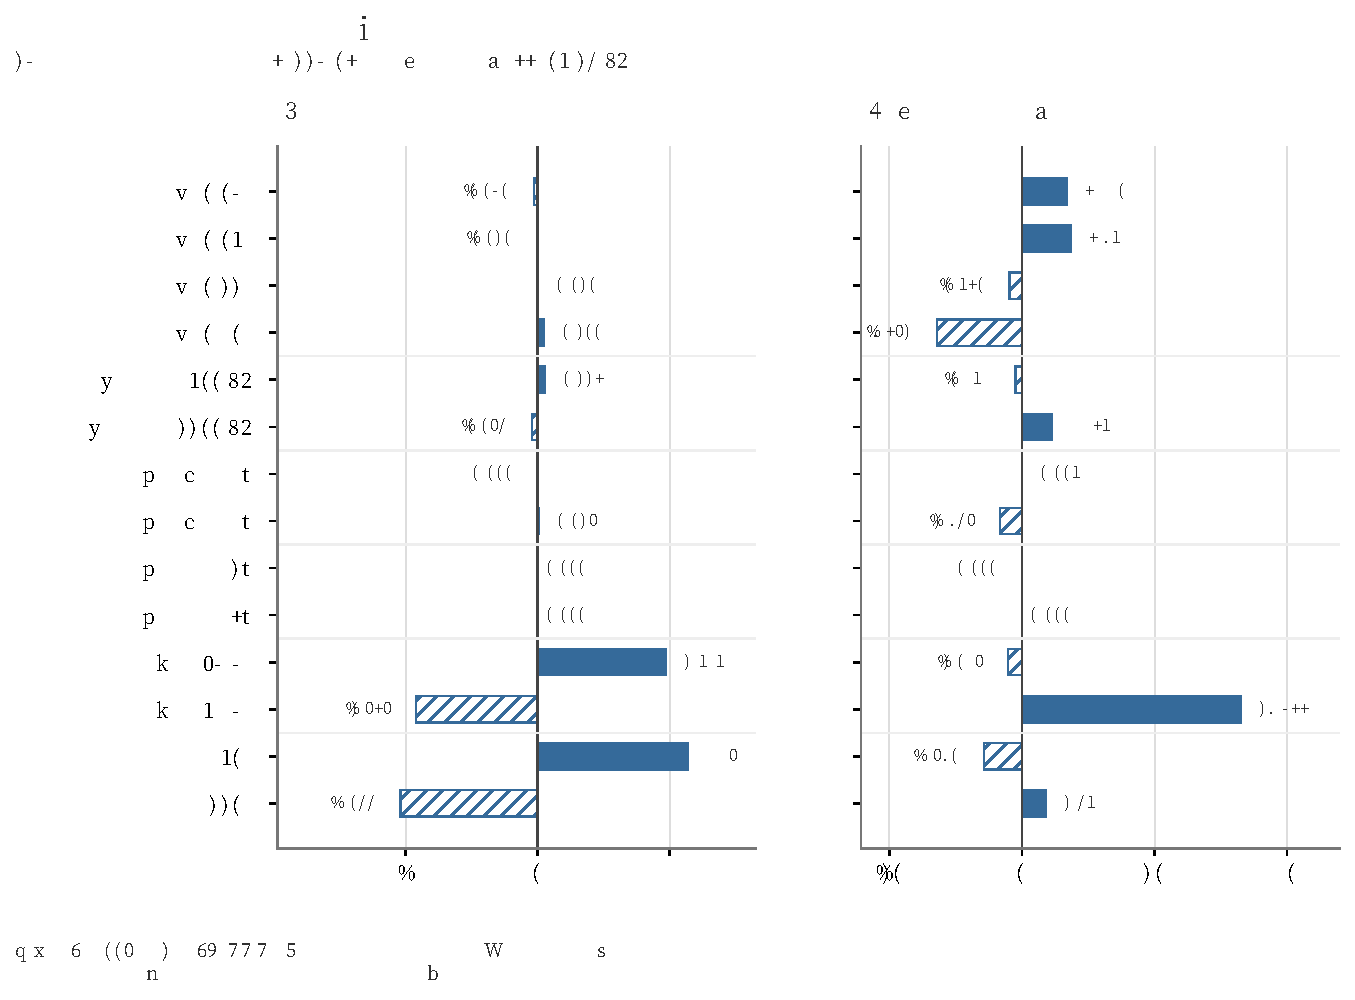
\includegraphics[width=\textwidth]{final_results/section9_visuals/q1_sensitivity.pdf}
 \caption{问题一单参数重求解的敏感性。变化率以基准方案为参照，实心与斜线分别表示增加和减少，两个面板采用不同横轴尺度。}
 \label{fig:section9-q1-sensitivity}
\end{figure}

图中结果体现了模型对物理条件的合理响应：提高储能效率或扩大容量能够降低购电费用，反向变化则增加费用，说明模型能够利用能量损耗与跨时段调配能力的变化调整策略。运行参数变化所引起的费用波动总体较小，且各组均保持可行，表明在本次考察范围内，方案对运行设置具有一定适应性。最短关闭时间变化几乎不影响结果，反映出该条件在当前典型日中并未成为限制调度的主要因素。

费用与平稳性两个面板同时说明了分层优化的必要性。适度放宽费用预算可以为降低功率波动提供空间，但效率提高带来的费用下降也可能伴随功率总变差增加，二者并非自然一致。模型通过明确的费用预算和运行要求协调这一矛盾，使平稳运行的代价能够被识别和控制。上述结果支持模型在所测参数范围内的有效性；其依据是单因素重新优化，结论限定于该典型日。

\subsection{第二问执行扰动的补充检验}
对先前完成的334日计划进行固定购电、固定模式的执行压力回放，以观察误差增大后电池反馈和紧急购电的作用。该试验保留当时的计划与起点，仅改变执行供需，逐槽连续传递储电量；未重新训练预测器或重新优化后续购电，也不将其费用当作本次全年冷启动策略的重训练检验。

乘性噪声取$\exp(\sigma z_t-\sigma^2/2)$，其中$z_t$为相关系数0.95的平稳AR(1)过程，负载与光伏两通道相关系数为$-0.3$，光伏零值保持为零。每个噪声幅度重复30次，使用相同随机数以比较不同强度，结果见图\ref{fig:section9-q2-stress}。
\begin{figure}[H]
 \centering
 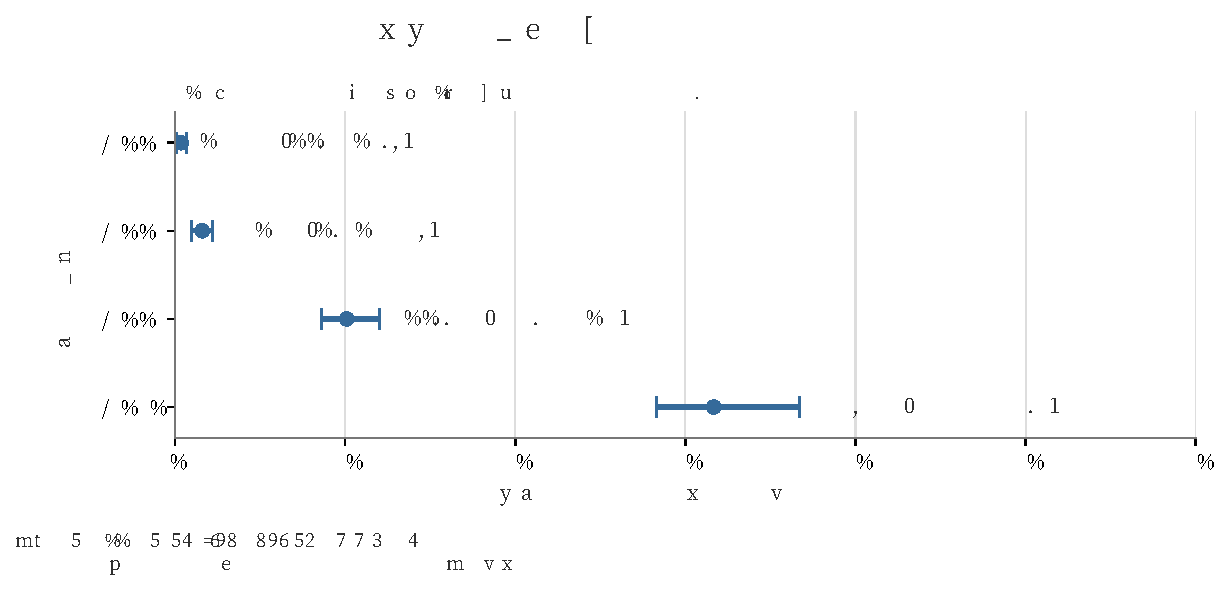
\includegraphics[width=\textwidth]{final_results/section9_visuals/q2_execution_stress.pdf}
 \caption{第二问历史固定计划的相关噪声执行回放。圆点为30次重复的费用平均变化，横线为5\%至95\%经验分位；该区间不表示未来实际费用的置信区间。}
 \label{fig:section9-q2-stress}
\end{figure}

较小扰动下，费用增幅及试验间差异均较有限，说明在无需改变既定购电计划的情况下，储能反馈与缺口补购机制能够使执行过程适应一定程度的供需偏差。这为模型在轻度预测偏差下的执行适应性提供了支持。扰动增强后，费用增幅明显扩大，经验分位区间也随之变宽，表明固定计划的经济缓冲能力存在边界，持续偏差会增加高价补购压力。

这一结果揭示了预测与反馈在模型中的不同作用：反馈负责在储能边界内响应当槽偏差，日前预测则影响后续补购的经济代价。外网可无限紧急补购的假设保障了模型中的负载供给，但费用恶化说明仅有物理可行性不足以保证经济性，也为后续引入预报更新与日内修正提供了动机。该试验支持的是所设扰动下固定计划的执行适应性，日内更新能够带来多少收益仍需由对应策略的比较结果判断。

\subsection{评价范围与求解精度}
问题一的循环总变差连接典型日首尾；年度非空反转删除空闲槽后统计相邻方向变化，涉及评价边界时按相应表注处理。计划模式变化预算与实际非空反转具有不同定义，不将8次预算直接当作实测次数。电芯等效满循环由电芯侧吞吐除以$2\times12000$计算。上述指标用于描述运行强度，不直接推导电池折旧或寿命。

混合整数规划的相对间隙描述该次代理问题的可行解与界，不代表年度实际费用误差。固定模式购电修正为局部数值优化，日内线性规划仅在本次发布的剩余时域求解；全年滚动执行不作全局最优性声明。年度数据参与过模型开发，本文保留合法信息截点和实际运行检验，不以单个随机种子或月度结果代替独立年份验证。
